\documentclass[ngerman]{gdb-aufgabenblatt}
\usepackage{enumitem}
\usepackage{dingbat}
\usepackage{ifsym}
\usepackage{amssymb}
\usepackage{amsmath}
\renewcommand{\Aufgabenblatt}{4}
\renewcommand{\Ausgabedatum}{Mi. 29.11.2017}
\renewcommand{\Abgabedatum}{Fr. 15.12.2017}
\renewcommand{\Gruppe}{Meimerstorf,Jochens,T�ter}
\renewcommand{\STiNEGruppe}{19}
\usepackage{tabularx}
\usepackage[normalem]{ulem}

\begin{document}

\section{Relationenalgebra}
\subsection{}
Die Nachnamen aller Matrosen, die auf einem Schiff anheuern, dessen Heimathafen Hamburg ist. \\
\subsection{}
$\pi_{Name,Stapellauf}((Matrose \verbund{MNR=Matrose} (\sigma_{Jahresgehalt>400000}anheuern) \verbund{Schiff=SNR} Schiff))$
\subsection{}
$\pi_{Nachname}\sigma_{Heimathafen=Ausbildungsort}((Matrose \verbund{MNR=Matrose} anheuern \verbund{Schiff=SNR} Schiff))$
\subsection{}
$\pi_{Grundsteinlegung}(Hafen\verbund{HNR=HNR}(\pi_{HNR}(Hafen) \setminus (\pi_{Ausbildungsort}(Matrose))))$
\section{Schemadefinition}
\begin{verbatim}
CREATE TABLE Person (
    Nachname VARCHAR(50) NOT NULL,
    Vorname VARCHAR(50) NOT NULL,
    Geburtsdatum DATE ,
    Wohnort VARCHAR(50) NOT NULL,
    Lieblingsbuch INT,
    BID INT, 
    CONSTRAINT prim_person  PRIMARY KEY(Nachname,Vorname),
    CONSTRAINT age_check CHECK(Geburtsdatum <  GETDATE())
);

CREATE TABLE Bibliothek (
    BID INT PRIMARY KEY,
    Name VARCHAR(50),
    Adresse VARCHAR(50),
	CONSTRAINT uq_name_adress UNIQUE(Name, Adresse),
	Leiter_Nachname VARCHAR(50) NOT NULL,
	Leiter_Vorname VARCHAR(50) NOT NULL,
	CONSTRAINT FK_PersonBibliothek FOREIGN KEY (Leiter_Nachname,Leiter_Vorname) REFERENCES Person(Nachname,Vorname)
);
ALTER TABLE Person
ADD CONSTRAINT fk_bib_person FOREIGN KEY (BID) REFERENCES Bibliothek(BID);

CREATE TABLE Buch (
    ISBN INT PRIMARY KEY,
    Titel VARCHAR(50),
    Autor_Nachname  VARCHAR(50) NOT NULL,
    Autor_Vorname  VARCHAR(50) NOT NULL,
    CONSTRAINT FK_Autor FOREIGN KEY (Autor_Nachname,Autor_Vorname) REFERENCES Person(Nachname,Vorname)
);

ALTER TABLE Person
ADD CONSTRAINT fk_lieblingsbuch FOREIGN KEY (Lieblingsbuch) REFERENCES Buch(ISBN);

CREATE TABLE leiht_aus (
	Vorname VARCHAR(50),
	Nachname VARCHAR(50),
	ISBN INT,
    CONSTRAINT FK_leightaus_Buch FOREIGN KEY (ISBN) REFERENCES Buch(ISBN),
    CONSTRAINT FK_leihtaus_person FOREIGN KEY (Nachname,Vorname) REFERENCES Person(Nachname,Vorname)
);
CREATE TABLE in_Bestand (
	BID INT NOT NULL,
	ISBN INT,
	Anzahl INT,
    CONSTRAINT FK_inBestand_Buch FOREIGN KEY (ISBN) REFERENCES Buch(ISBN),
    CONSTRAINT FK_inBestand_Bib FOREIGN KEY (BID) REFERENCES Bibliothek(BID),
    CONSTRAINT Anzahl_Check Check(Anzahl>1)
);
\end{verbatim}

\section{SQL}
\subsection{}
\begin{verbatim}
SELECT DISTINCT m1.Geburtsdatum
FROM Matrose m1, Schiff s1, anheuern a1
Where m1.MNR = a1.Matrose 
AND a1.Schiff = s1.SNR 
AND a1.Dienstbeginn = '1957-04-01'
ORDER BY m1.Geburtsdatum DESC
\end{verbatim}
\subsection{}
\begin{verbatim}
SELECT *
FROM Matrose
Where Geburtsdatum > '1530-01-01' 
AND Geburtsdatum < '1535-01-01' 
AND Nachname LIKE 'H%'
\end{verbatim}
\subsection{}
\begin{verbatim}
SELECT m1.MNR,m1.Nachname,MAX(a1.Jahresgehalt)
FROM Matrose m1, anheuern a1
Where m1.MNR = a1.Matrose
GROUP BY a1.Matrose
\end{verbatim}
\subsection{}
\begin{verbatim}
SELECT h.Ort
FROM Hafen h
WHERE h.HNR NOT IN (
SELECT s.Heimathafen
FROM Schiff s)
\end{verbatim}
\subsection{}
\begin{verbatim}
SELECT m.MNR, a1.Jahresgehalt
FROM Matrose m, anheuern a1, Schiff s1
WHERE m.MNR = a1.Matrose AND a1.Schiff = s1.SNR AND a1.Dienstbeginn < '2016-12-24'
GROUP BY m.MNR
HAVING MAX(a1.Jahresgehalt) < 40000
\end{verbatim}
\subsection{}
Der Ort des Hafens, an dem zwei Schiffe mit unterschiedlichen Heimath�fen am selben Tag Stapellauf hatten.
\section{}
\subsection{}
\subsubsection{Unoptimiert:}
\begin{center}
\begin{tikzpicture}[scale=0.2]
\tikzstyle{every node}+=[inner sep=0pt]
\draw (6,-48.3) node {$Matrose$};
\draw (17.6,-47.5) node {$Anheuern$};
\draw (33.6,-47.5) node {$Schiff$};
\draw (10.9,-37.1) node {$\times$};
\draw (27.5,-31.5) node {$\times$};
\draw (27.5,-23) node {$\sigma_{Schiff=SNR}$};
\draw (27.5,-15.1) node {$\sigma_{MNR=Matrose}$};
\draw (27.5,-8) node {$\sigma_{Heimathafen=15}$};
\draw (27.5,-0.6) node {$\pi_{Ausblidungsort}$};
\draw [black] (7.2,-45.55) -- (9.7,-39.85);
\draw [black] (15.98,-44.98) -- (12.52,-39.62);
\draw [black] (13.74,-36.14) -- (24.66,-32.46);
\draw [black] (32.53,-44.7) -- (28.57,-34.3);
\draw [black] (27.5,-28.5) -- (27.5,-26);
\draw [black] (27.5,-12.1) -- (27.5,-11);
\draw [black] (27.5,-5) -- (27.5,-3.6);
\draw [black] (27.5,-20) -- (27.5,-18.1);
\end{tikzpicture}
\subsubsection{Optimiert:}

\begin{center}
\begin{tikzpicture}[scale=0.2]
\tikzstyle{every node}+=[inner sep=0pt]
\draw (6,-48.3) node {$Matrose$};
\draw (18.3,-48.3) node {$Anheuern$};
\draw (33.6,-47.5) node {$Schiff$};
\draw (33.6,-39.2) node {$\sigma_{Heimathafen=15}$};
\draw (12.4,-38) node {$\times$};
\draw (12.4,-29.9) node {$\sigma_{MNR=Matrose}$};
\draw (25.6,-24.5) node {$\times$};
\draw (25.6,-16.6) node {$\sigma_{Schiff=SNR}$};
\draw (25.6,-8) node {$\pi_{Ausbildungsort}$};
\draw [black] (7.58,-45.75) -- (10.82,-40.55);
\draw [black] (16.81,-45.7) -- (13.89,-40.6);
\draw [black] (12.4,-35) -- (12.4,-32.9);
\draw [black] (33.6,-44.5) -- (33.6,-42.2);
\draw [black] (15.18,-28.76) -- (22.82,-25.64);
\draw [black] (32.17,-36.56) -- (27.03,-27.14);
\draw [black] (25.6,-21.5) -- (25.6,-19.6);
\draw [black] (25.6,-13.6) -- (25.6,-11);
\end{tikzpicture}
\end{center}
\end{center}
\subsection{Optimierter Operatorbaum mit Kardinalit�ten}
\begin{center}
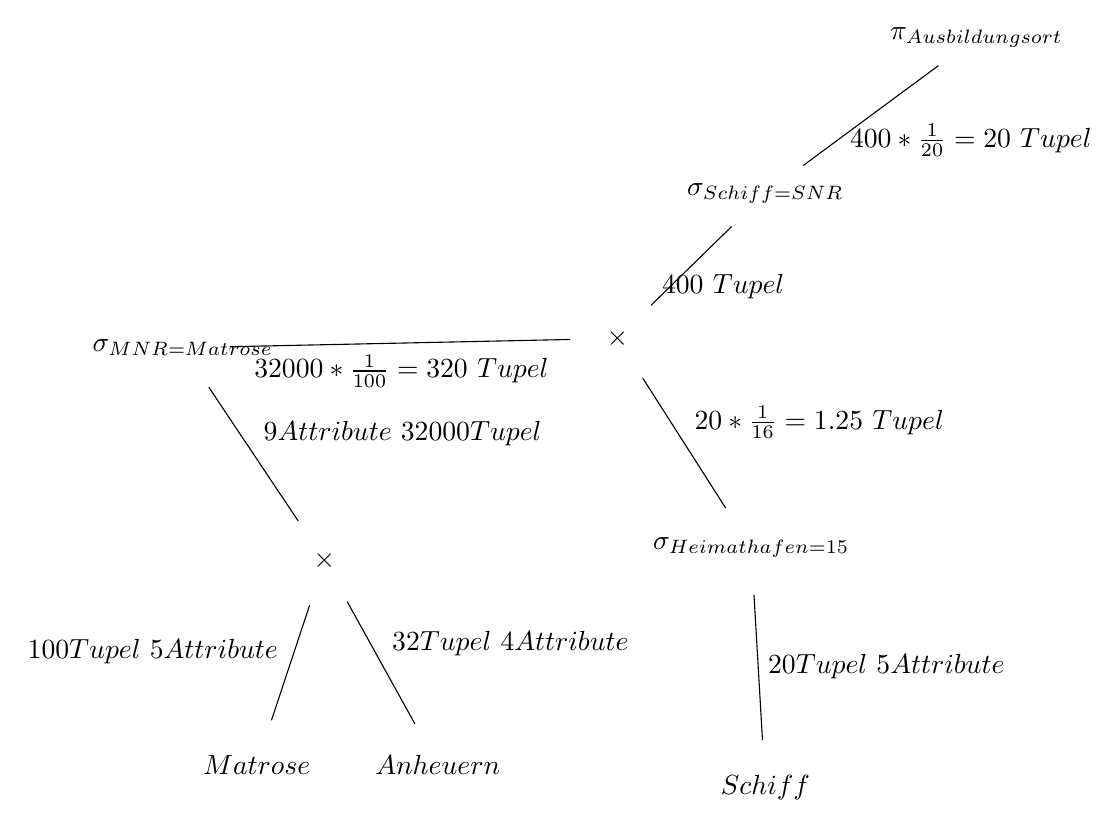
\begin{tikzpicture}[scale=0.2]
\tikzstyle{every node}+=[inner sep=0pt]
\draw (11.5,-51) node {$Matrose$};
\draw (23,-51) node {$Anheuern$};
\draw (43.8,-52.4) node {$Schiff$};
\draw (42.9,-37.2) node {$ \sigma_{Heimathafen=15}$};
\draw (15.8,-38) node {$\times$};
\draw (6.8,-24.5) node {$\sigma_{MNR=Matrose}$};
\draw (34.4,-23.9) node {$\times$};
\draw (43.8,-14.7) node {$\sigma_{Schiff=SNR}$};
\draw (57.2,-4.8) node {$\pi_{Ausbildungsort}$};
\draw [black] (12.44,-48.15) -- (14.86,-40.85);
\draw (12.88,-43.8) node [left] {$100Tupel \ 5 Attribute$};
\draw [black] (21.55,-48.38) -- (17.25,-40.62);
\draw (20.07,-43.3) node [right] {$32 Tupel \ 4  Attribute$};
\draw [black] (14.14,-35.5) -- (8.46,-27);
\draw (11.91,-29.92) node [right] {$9 Attribute \ 32000 Tupel$};
\draw [black] (43.62,-49.41) -- (43.08,-40.19);
\draw (43.94,-44.77) node [right] {$20 Tupel \ 5 Attribute$};
\draw [black] (9.8,-24.43) -- (31.4,-23.97);
\draw (20.69,-24.89) node [below] {$32000 *\frac{1}{100}=320 \ Tupel$};
\draw [black] (41.28,-34.67) -- (36.02,-26.43);
\draw (39.27,-29.24) node [right] {$20*\frac{1}{16}=1.25 \ Tupel$};
\draw [black] (36.54,-21.8) -- (41.66,-16.8);
\draw (41.12,-19.78) node [below] {$400 \ Tupel$};
\draw [black] (46.21,-12.92) -- (54.79,-6.58);
\draw (56.85,-10.25) node [below] {$400*\frac{1}{20}=20 \ Tupel$};
\end{tikzpicture}
\end{center}
 
\end{document}